
\documentclass{article}
\usepackage[margin=2cm]{geometry}
\usepackage[dvips]{graphicx}
\begin{document}

\section*{Learning goals}
\label{sec:learning-goals}

Before the next day, you should have achieved the following learning
goals: 

\begin{itemize}
\item Understand how to use interfaces in Java, and use them in your
  programs. 
\item Understand how trees work.
\item Strengthen your understanding of pointers, and how they are used
  in dynamic data structures. 
\item Strengthen your understanding of interfaces, and how they are used
  to separate public behaviour from hidden implementation. 
\end{itemize}

You should be able to finish most of non-star exercises in the lab. 
Remember that star exercises are more difficult. 
\textbf{Do not try star-exercises unless the other ones are clear to
  you}.  

\section{Integer Binary Tree}
\label{sec:queues}

\subsection{First steps: add and seek}
\label{sec:first-steps:-add}

Complete the class \verb+IntegerTreeNode+. 

From the notes, you already know what the member fields are and you
have seen a possible implementation of methods \verb+add(int)+ and
\verb+contains(int)+. Implement as well two methods \verb+getMax()+
and \verb+getMin()+ that returns the maximum and the minimum values
stored in the tree. 

Compile the class and use it inside a script\footnote{In Java, a script
  is a class that only contains a main() method, maybe a launch()
  method, and no member fields.} adding numbers in different
orderings. 

\subsection{Tree traversal}
\label{sec:tree-traversal}

Add a method \verb+toString()+ to the class. This methods must return
a representation of your tree in String form, where every node is
represented as a list in square brackets containing its value, the
left branch, and the right branch; the left branch should be prefixed
by ``L'' and the right branch by R, and an empty branch should be
shown as an empty pair of square brackets. 
Some examples of outputs in Figure~\ref{fig:jdjfj}.

After you have commited this version of \verb+toString()+, make
another version that returns a simplified representation, where every
node is represented as a list in square brackets containing its value
and its branches, but only if they are not empty; without using the
``L'' and ``R'' prefixes. 
Some examples of outputs in Figure~\ref{fig:jdjfj}.

Check that both versions of the method work by adding several elements
and printing the String representation of the tree. 

\begin{figure}[hbtp]
  \centering
  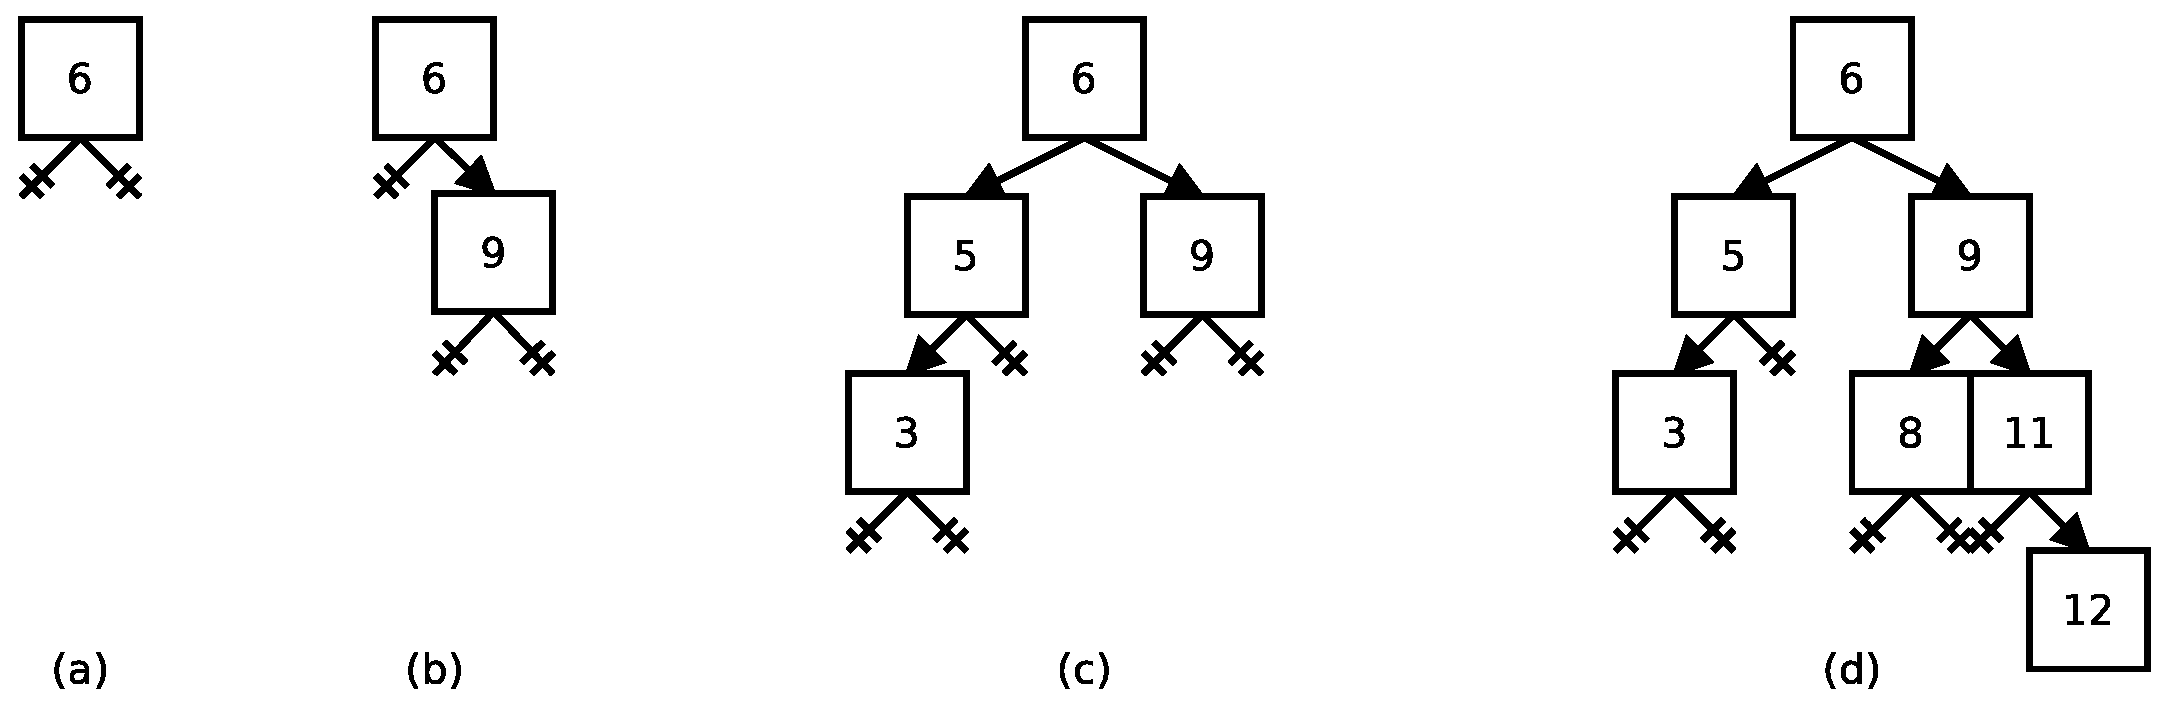
\includegraphics[width=\textwidth]{gfx/tree-toString}
  \begin{tabular}{ll}
      & Complete \\
    a & [6 L[] R[]] \\
    b & [6 L[] R[9 L[] R[]]] \\
    c & [6 L[5 L[3 L[] R[]] R[]] R[9 L[] R[]]] \\
    d & [6 L[5 L[3 L[] R[]] R[]] R[9 L[8 L[] R[]] R[11 L[] R[12 L[] R[]]]]] \\
      & Simplified \\
    a & [6] \\
    b & [6 [9]] \\
    c & [6 [5 [3]] [9]] \\
    d & [6 [5 [3]] [9 [8] [11 [12]]]] \\
  \end{tabular}
  \caption{Several trees and their String representations, both in
    complete form and in simplified form.}
  \label{fig:jdjfj}
\end{figure}

\subsection{Depth}
\label{sec:depth}

Add a method \verb+depth()+ that returns the number of levels in a
tree. By convention, a tree with only one node (i.e.~the root) has a
depth of zero. Hint: the depths of the trees in Figure~\ref{fig:jdjfj}
are 0, 1, 2, and 3. 

Hint: the depth of a tree is one more than the deepest of its
subtreees. 

\subsection{Deletion of elements (*)}
\label{sec:deletion-elements}

Add a method \verb+remove(int)+ to the class. This method must look
for the node that contains the given value and remove it from the
tree. 

Hint: removing leafs is trivial; to remove nodes, you can replace the
removed node with its highest element on its left or the lowest on its
right. 

\subsection{Rebalancing a tree (**)}
\label{sec:rebalancing-tree-}

Trees work very well with unsorted data because they automatically
sort it as they are filled up with data. There is a problem with
already sorted data, though: all elements are placed on the same
branches and the ``natural sorting'' effect is lost, the tree becomes
just a list with an additional null pointer at every level. 

Add a method \verb+rebalance()+ to your tree that re-arranges the tree
to make it balanced, i.e.~having approximately the same number of
nodes on both branches. 


\section{Trees as sets}
\label{sec:trees-as-sets}

A set is a collection of elements that does not contain duplicates. 

\subsection{Interface}
\label{sec:interface1}

Create an \emph{interface} \verb+IntSet+ with the following methods,
including the comments: 

\begin{description}
\item[add(int)] adds a new \emph{int} to the set; if it is there
  already, nothing happens.
\item[contains(int)] returns true if the number is in the set, false
  otherwise.
\item[containsVerbose(int)] returns the same values as the former
  method, but for every element that is checked prints its value on
  screen.
\item[toString()] returns a string with the values of the elements in
  the set separated by commas.
\end{description}

\subsection{Implementation as tree}
\label{sec:impl-as-tree1}

Create a class \verb+TreeIntSet+ that implements this interface based
on a tree structure. 

\subsection{Implementation as list}
\label{sec:impl-as-list1}

Create a class \verb+ListIntSet+ that implements this interface based
on a linked list structure. 


\section{Trees as (sorted) lists}
\label{sec:trees-as-lists}

\subsection{Interface}
\label{sec:interface}

Create an \emph{interface} \verb+IntSortedList+ with the following methods,
including the comments: 

\begin{description}
\item[add(int)] adds a new \emph{int} to the list so that the list
  remains sorted; a list can contain duplicates unlike a set.
\item[contains(int)] returns true if the number is in the list, false
  otherwise.
\item[toString()] returns a string with the values of the elements in
  the list separated by commas.
\end{description}

\subsection{Implementation as tree}
\label{sec:impl-as-tree}

Create a class \verb+TreeIntSortedList+ that implements this interface based
on a tree structure. 

\subsection{Implementation as list}
\label{sec:impl-as-list}

Create a class \verb+ListIntSortedList+ that implements this interface based
on a linked list structure. 


\section{Abstract syntax tree (*)}
\label{sec:abstract-tree-}

When a computer reads a mathematical expression (or a program), the
first step in understanding it is creating a tree representation. The
nodes contain the operations and the leaves contain the operands. 

Create a binary tree node class, where each node contains a
String. Apart from the usual \emph{add(String)} and \emph{toString()}
methods, add a static method that takes a mathematical expression as a
String and returns a tree that represents the mathematical
expression. 

\begin{figure}[hbtp]
  \centering
  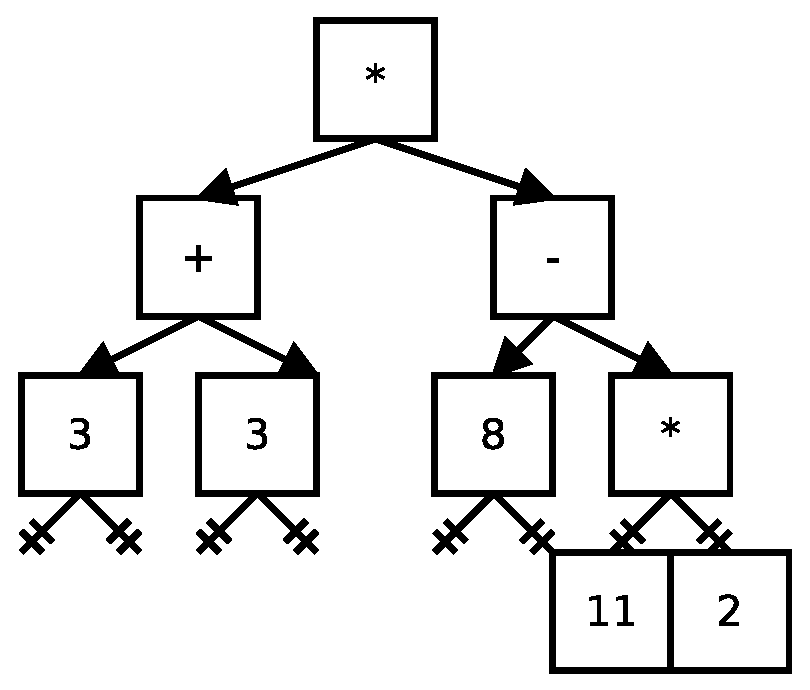
\includegraphics[width=8cm]{gfx/tree-operation}
  \caption{Example of tree representing a mathematical expression: "(3 + 3) * (8 - 11 * 2)".}
  \label{fig:jjgg}
\end{figure}

\section{Git internals (**)}
\label{sec:git-internals}

In this exercise you will create a simplified representation of a source
control tree similar to the way Git does it. 

Nodes (commits) in your tree will have three fields: an integer ID, a String
description, and a list of parents. This list can be arbitrarily long:
use an interface List with an only method \verb+add()+ (there can be
no deletions of parents), then implement it by using pointers or
arrays as you did in the exercises of Day 7. 

\begin{verbatim}
    public class CommitNode {
        private int ID;
        private String description;
        private CommitNodeList parentList;
        // ...methods come here...
    }
\end{verbatim}

\begin{verbatim}
    public interface CommitNodeList {
        void add(CommitNode newCommit);
    }
\end{verbatim}

The code does not show the comments for the sake of space, but your
code should have proper comments. You will need at least two auxiliary
pointers to commit nodes, and may 
have many more (i.e.~you will need a list of pointers to commit nodes
called something like \verb+branchList+): 

\begin{description}
\item[HEAD. ] This pointer points to the current commit (not
  necessarily the most recent one, see ``checkout'' and ``change
  branch'' below).
\item[MASTER (and other branches).] Branches are just pointers to
  commits. 
\end{description}

Your program should request commands from the user, and act
accordingly: 

\begin{description}
\item[Commit. ] Adds a new commit to the current branch if the current
  branch and HEAD point to the same commit. If not, nothing happens
  (except maybe an error message on screen). 
  The ID must be assigned automatically but the message is decided by
  the user.  
  The new commit is linked to its parent (the former HEAD). 
\item[Checkout. ] Moves HEAD to point to another commit, as provided
  by the ID. If the ID does not exist, nothing happens
  (except maybe an error message on screen). 
  The current branch does not change. 
\item[Create branch. ] Creates a new branch, which means adding a new
  commit-pointer to the list of pointers (\verb+branchList+) and 
  make it point to HEAD. 
  The current branch does not change. 
\item[Change branch. ] Similar to checkout. Moves HEAD to point to
  another commit as provided by the branch name. Then changes current
  branch to that one. 
\item[Merge. ] Creates a new commit (with a new ID and new
  description), whose parents are the current branch and all the other
  branches provided (by their names). Only works if current branch and
  HEAD point to the same commit, otherwise nothing happens
  (except maybe an error message on screen). 
  The current branch does not change. 
\end{description}

The diagrams at
http://git-scm.com/book/en/Git-Branching-Basic-Branching-and-Merging
may be of help. 

\end{document}